\documentclass[12pt]{amsart}


\usepackage{times}
\usepackage[margin=0.7in]{geometry}
\usepackage{paralist,amsmath,amssymb,multicol,graphicx,framed,ifthen,color,xcolor,stmaryrd,enumitem,colonequals}
\usepackage{tikz}
\usepackage[outline]{contour}
\contourlength{.4pt}
\contournumber{10}
\newcommand{\Bold}[1]{\contour{black}{#1}}

\definecolor{chianti}{rgb}{0.6,0,0}
\definecolor{meretale}{rgb}{0,0,.6}
\definecolor{leaf}{rgb}{0,.35,0}
\newcommand{\Q}{\mathbb{Q}}
\newcommand{\N}{\mathbb{N}}
\newcommand{\Z}{\mathbb{Z}}
\newcommand{\R}{\mathbb{R}}
\newcommand{\C}{\mathbb{C}}
\newcommand{\e}{\varepsilon}
\newcommand{\inv}{^{-1}}
\newcommand{\dabs}[1]{\left| #1 \right|}
\newcommand{\ds}{\displaystyle}
\newcommand{\solution}[1]{\ifthenelse {\equal{\displaysol}{1}} {\begin{framed}{\color{meretale}\noindent #1}\end{framed}} { \ }}
\newcommand{\solutione}[1]{\ifthenelse {\equal{\displaysol}{1}} {\begin{framed}{\color{leaf}This solution is embargoed.}\end{framed}} { \ }}
\newcommand{\showsol}[1]{\def\displaysol{#1}}

\newcommand{\rsa}{\rightsquigarrow}


\newcommand\itemA{\stepcounter{enumi}\item[{\Bold{(\theenumi)}}]}
\newcommand\itemB{\stepcounter{enumi}\item[(\theenumi)]}
\newcommand\itemC{\stepcounter{enumi}\item[{\it{(\theenumi)}}]}
\newcommand\itema{\stepcounter{enumii}\item[{\Bold{(\theenumii)}}]}
\newcommand\itemb{\stepcounter{enumii}\item[(\theenumii)]}
\newcommand\itemc{\stepcounter{enumii}\item[{\it{(\theenumii)}}]}
\newcommand\itemai{\stepcounter{enumiii}\item[{\Bold{(\theenumiii)}}]}
\newcommand\itembi{\stepcounter{enumiii}\item[(\theenumiii)]}
\newcommand\itemci{\stepcounter{enumiii}\item[{\it{(\theenumiii)}}]}
\newcommand\ceq{\colonequals}


\DeclareMathOperator{\ord}{ord}

\DeclareMathOperator{\res}{res}
\setlength\parindent{0pt}
%\usepackage{times}

%\addtolength{\textwidth}{100pt}
%\addtolength{\evensidemargin}{-45pt}
%\addtolength{\oddsidemargin}{-60pt}

\pagestyle{empty}
%\begin{document}\begin{itemize}

%\thispagestyle{empty}




\begin{document}
\showsol{0}
	
	\thispagestyle{empty}
	
	\section*{Dihedral Groups}
	
	

\begin{framed}
\textsc{Definition:}
\begin{itemize}
\item A \textbf{isometry} of $\mathbb{R}^2$ is a bijective function $f:\mathbb{R}^2 \to \mathbb{R}^2$ that preserves distances between pairs of points; examples include rotations around a point, translations, and reflections over a line.

\item Let $X\subseteq \mathbb{R}^2$. A \textbf{symmetry} of $X$ is an isometry of $\mathbb{R}^2$ such that $f(X)=X$ as a set.

\item The \textbf{dihedral group} $D_n$ is the group of symmetries of a regular $n$-gon $P_n$ in the plane, with composition of functions as the group operation.
\end{itemize}


\


\textsc{Theorem 1:} The dihedral group $D_n$ is indeed a group. It has exactly $2n$ elements consisting of:
\begin{itemize} 
\item The identity map $e$,
\item $n-1$ rotations $r, r^2, \dots, r^{n-1}$, where $r$ is counterclockwise rotation by $2\pi/n$ (so $r^j$ is counterclockwise rotation by $2\pi j/n$),
\item $n$ reflections. More precisely, 
\begin{itemize} 
\item for $n$ is odd, there are $n$ distinct reflections over lines between a vertex and opposite edge;
\item for $n$ is even, there are $n/2$ distinct reflections over lines between opposite pairs of vertices, and another $n/2$ distinct reflections over lines between opposite pairs of edges.
\end{itemize}
\end{itemize}

\begin{center}
\begin{minipage}{0.4\textwidth}
\begin{center}
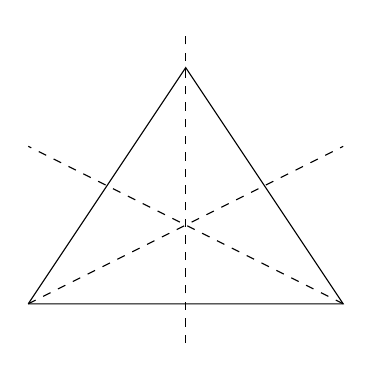
\begin{tikzpicture}
\draw (0,0) -- (2,3) -- (4,0) -- (0,0);
\draw[dashed] (2,-0.5) -- (2,3.5);
\draw[dashed] (0,0) -- (4,2);
\draw[dashed] (4,0) -- (0,2);
\end{tikzpicture}

\vspace{2.4em}

The reflection lines in $D_3$
\end{center}
\end{minipage}
\begin{minipage}{0.4\textwidth}
\begin{center}
\begin{tikzpicture}
\draw (0,0) -- (4,0) -- (4,4) -- (0,4) -- (0,0);
\draw[dashed] (2,-0.5) -- (2,4.5);
\draw[dashed] (-0.5,2) -- (4.5,2);
\draw[dashed] (-0.3,-0.3) -- (4.3,4.3);
\draw[dashed] (-0.3,4.3) -- (4.3,-0.3);
\end{tikzpicture}

The reflection lines in $D_4$
\end{center}
\end{minipage}
\end{center}

\vspace{0.5em}


\end{framed}

\begin{enumerate}

\itemA Why is the dihedral group a group? I.e., why are the group axioms true for this set and operation?

\

\itemA What is the order of the rotation $r$? What is the order of a reflection in $D_n$?

\

\itemB Proof of Theorem 1:
\begin{enumerate}
\itemb Show that\footnote{Hint: After rescaling, we can assume that $d(c,v)=1$ for any vertex $v$. Then observe that
\begin{enumerate}  \item $d(c,x)\leq 1$ for any $x\in P_n$, and
\item if $q\in P_n$ is \emph{not} the center, then $d(q,x) >1$ for some $x\in P_n$.
\end{enumerate}} if  $f$ is a symmetry of $P_n$ and $c$ is the center of $P_n$, then $f(c)=c$. 
\itemb Show that\footnote{Hint: Again assume $d(c,v)=1$ for any vertex $v$. Observe that $v$ is a vertex of $P_n$ if and only if $d(c,v)=1$.}
 if $f$ is a symmetry of $P_n$ and $v$ is a vertex of $P_n$, then $f(v)$ is a vertex of $P_n$.
\itemb Show that if $f$ is a symmetry of $P_n$ and $v,v'$ are adjacent vertices, then $f(v)$ and $f(v')$ are adjacent vertices of $P_n$.
\itemb Prove\footnote{You can use the following fact from geometry: if $f,f'$ are two isometries of the plane, $p_1,p_2,p_3 \in \mathbb{R}^2$ are three points not on a line, and $f(p_i)=f'(p_i)$ for $i=1,2,3$, then $f=f'$.} the Theorem.
\end{enumerate}
\end{enumerate}



\begin{framed}

\textsc{Lemma:} Let $v\in P_n$ be a vertex, and $s\in D_n$ the reflection through the axis containing $v$. Let $r\in D_n$ be counterclockwise rotation by $2\pi/n$. Then $s r s = r^{-1}$.


\

\textsc{Theorem 2:} Let $v\in P_n$ be a vertex, and $s\in D_n$ the reflection through the axis containing $s$. Let $r\in D_n$ be counterclockwise rotation by $2\pi/n$.
\begin{enumerate}
\item Every element of $D_n$ can be written uniquely in the form 
\[ r^j \quad \text{for} \ j=0,\dots,n-1, \qquad \text{or} \qquad r^j s \quad \text{for} \ j=0,\dots,n-1.\]
\item $D_n$ is generated by $r,s$.
\item $D_n$ has the group presentation $\langle r,s \ | \ r^n=e, s^2=e, srs^{-1} = r^{-1}\rangle$.
\end{enumerate}
\end{framed}

\

\begin{enumerate}
\setcounter{enumi}{3}
\itemA Show that the elements $r^j s$ for $j=0,\dots,n-1$ are $n$ distinct reflections. Deduce Theorem 2(1) from this and Theorem 1.

\

\itemA Use the Theorem 2(1) to prove Theorem 2(2).

\

\itemB Prove the Lemma. 

\

\itemB Discuss Theorem 2(3).

\

\hrulefill

\

\itemB Consider a circle in the plane. 
\begin{enumerate}
\itemb Compute the symmetry group $G$ of the circle; give an answer in a similar form to Theorem 1.
\itemb What are all of the possible orders of elements in this group?
\itemb Find two elements of order $2$ in $G$ whose product has infinite order.
\itemb Does $G$ has a finite generating set?
\end{enumerate}




\end{enumerate}











\end{document}
